\section*{Introduction}~\label{chapIntroduction}
Engineering as a practice has always centered around finding optimized solutions for real-world applications. Throughout history, countless names have devoted their efforts towards developing mathematical tools and models that allowed the next generation of engineers to further expand the knowledge over physical phenomena. Paired with the rapid increase in computing capacity seen over the last few decades, there is a duty to continue their work with the new tools available in our time. In the field of Computer Fluid Dynamics and Heat Transfer (CFD \& HT), the resolution of the Navier-Stokes equations presents an important challenge that can be optimized for a wide variety of industrial applications. The Navier-Stokes (NS) equations describe the motion of viscous fluids and the complex interactions involved in the phenomena by evaluating the conservation of mass, momentum and energy. However, NS equatios are non-linear since the velocity and pressure equations (velocity \& mass) in the system are mutually dependent. This adds a layer of complexity for solving the system of equations and in consequence there is no general solution that can be directly solved. However, all conservation equations follow the same physical principle that describes transport phenomena.

This report will cover the development of numerical tools for the resolution of Convection-Diffusion problems while consolidating the knowledge related to the transport phenomena and the application of numerical methods for their resolution. The spatial discretization in this project will follow a finite volume method to discretize the analyzed domain into a finite amount of control volumes. The model will be developed in stages of increasing complexity, starting with pure diffusion, convection-diffusion, and finally coupled NS problems; using well-known benchmarks to validate the obtained results at each stage. During the development, the effect of the different numerical parameters involved in the model will be studied to further understand the mathematical implications of using a numerical tools like the one proposed with this project. Furthermore, the nature of each different case will require the implementation of different numerical solver algorithms that address the optimization problem in different manners.


\subsection*{Finite Volume Method (FVM)}
As mentioned above, the model will separate the domain into rectangular control volumes, which will then be evaluated independently considering all their interactions with the adjacent nodes or boundaries. Figure~\ref{figMeshDiagram} shows the representation of an interior node surrounded by adjacent nodes on all sides. As it can be seen, the four neighbours will be assigned a letter corresponding to their cardinal direction, using capital letters to refer to values located at the adjacent node centroid, and uncapitalized letters to refer to values located at the interface between the main node and the respective adjacent node. This presents some particular dificulties, as values are only known at the node centroids, and different schemes for interpolation may be used to estimate the values at the interface for certain models.

\begin{figure}[ht]
    \centering
    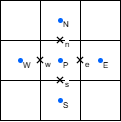
\includegraphics[width=0.25\linewidth]{Media/MeshDiagram.png}
    \caption{Node distribution for a single control volume $P$. Subindexes for each adjacent node correspond to their cardinal direction relative to the main node. Using the capitalized letter to represent values located at the adjacent node centroid ($W$, $E$, $S$, $N$) and the uncapitalized alternative for values located at the wall corresponding to the interaction between the main node and the adjacent node.}
    \label{figMeshDiagram}
\end{figure}


\subsection*{Governing Transport Equations}
When studying transport phenomena, there are two main mechanisms that govern the propagation of a transport variable $\phi$. These are known as \textbf{Convection} and \textbf{Diffusion}, and classify the phenomena depending on what causes the transport of the transport variable $\phi$. Diffusion refers to transport caused by molecular movement within the body, while Convection refers to transport caused by bulk movement of the body. The governing transport equation for this phenomena is given by Eq.~\eqref{eqTransGov}, which is separated into four terms relating to the physical variation of $\phi$. The accumulation term describes the magnitude variation over time, the convective term describes the variation due to convection, the diffusive term describes the variation due to diffusion, and the source term describes any additional source contributions.

\begin{equation} \label{eqTransGov}
    \overbrace{\frac{\partial (\rho \phi)}{\partial t}}^{\text{Accumulation}} + \overbrace{\nabla (\rho v \phi)}^{\text{Convective}} = \overbrace{\nabla (\Gamma \nabla \phi)}^{\text{Diffusive}} + \overbrace{S_{P}}^{\text{Source}}
\end{equation}

The continuous governing equation needs to be integrated over a control volume $V_P$ with a defined time-step $\Delta t$. By applying the Gauss divergence theorem shown in Eq.~\ref{eqGaussDivergence}, the convective and diffusive terms can be converted into surface integrals, which will evaluate the flow through the cell interface.

\begin{equation}~\label{eqGaussDivergence}
    \int_{V_P} \frac{\partial (\rho \phi)}{\partial t} \, dV = \oint_{\partial V_P} \rho \mathbf{v} \phi \cdot \hat{n} \, dA = \oint_{\partial V_P} \Gamma \nabla \phi \cdot \hat{n} \, dA + \int_{V_P} S_P \, dV
\end{equation}

Each surface integral can then be approximated as a discrete sum over the four cell faces (west, east, south, north). The resulting discretized forms are shown by Eqs.~\eqref{eqTransAcc}--\eqref{eqTransConv}

\begin{equation}~\label{eqTransAcc}
	\frac{\partial (\rho \phi)}{\partial t} = \rho \frac{\phi_P - \phi^0_P}{\Delta t}
\end{equation}

The accumulation term follows a first-order implicit approximation, where $\phi^0_P$ corresponds to the value of node $P$ at the current time-step and $\phi_P$ corresponds to the value at the next time-step.

\begin{equation}~\label{eqTransDiff}
    \oint_{\partial V_P} \Gamma \nabla \phi \cdot \hat{n} \, dA = \Gamma_w \frac{\phi_W - \phi_P}{d_{PW}} S_w - \Gamma_e \frac{\phi_P - \phi_E}{d_{PE}} S_e + \Gamma_s \frac{\phi_S - \phi_P}{d_{PS}} S_s - \Gamma_n \frac{\phi_P - \phi_N}{d_{PN}} S_n
\end{equation}

The diffusive term approximates the gradient at the face by interpolating the values from the adjacent nodes, multiplied by the diffusivity coefficient $\Gamma$ and the surface at the interface $S_k$, and dividing by the distance between the central node and one of the adjacent nodes $d_{PK}$.

\begin{equation}~\label{eqTransConv}
    \oint_{\partial V_P} \rho \mathbf{v} \phi \cdot \hat{n} \, dA = \rho (v_e \phi_E S_e - v_w \phi_W S_w + v_n \phi_N S_n - v_s \phi_S S_s)
\end{equation}

The convective term uses the velocity components located at the cell wall faces, considered in the expression with their corresponding geometrical surface value. For this term, the convective scheme can considerably change the behaviour of the model.

By substituting all previously mentioned equations and organizing the different terms, the expression can be reorganized to depend only on the magnitude of the current node $P$ and its neighbours. Eq.~\eqref{eqTransDisc} shows the standard FVM form for an interior cell with 4 adjacent nodes.

\begin{equation}~\label{eqTransDisc}
    a_P \phi_P = a_W \phi_W + a_E \phi_E + a_S \phi_S + a_N \phi_N + b_P
\end{equation}

The coefficients $a_W, a_E, a_S, a_N$ include the effect of both the diffusive and convective phenomena. When using this discretization, the coefficient for the current cell $a_P = a_W + a_E + a_S + a_N + a^0_P$ will respect diagonal dominance due to the presence of the accumulation term $a^0_P = \rho V_P / \Delta t$. This equation will be iteratively solved for every node in the discretized domain at each time-step. Each chapter will include a brief explanation of the specific expressions used for each coefficient for their respective application. 


\subsection*{Motivation}


\subsection*{Objectives}
\begin{enumerate}
    \item{Develope a modular FVM solver using C++ capable of accurately simulating transport phenomena of increasing complexity. Using several benchmark cases to validate the accuracy of the implementation at each stage of the model, and testing the performance and behaviour of the different numerical methods implemented in the model once validated.}
    \item{Expand the knowledge about numerical methods applied to CFD \& HT and use it to solve and understand the resolution methodology of complex transport phenomena. Simultaneously using the opportunity to further develope a consistent and organized code structure and learning more about C++ and its capabilities as a programming language.}
\end{enumerate}


\subsection*{Scope}
The model developed in this project will solve three main models, testing a variety of benchmark problems for each one of them.

\begin{enumerate}
    \item The \textbf{pure diffusion} model will evaluate a purely diffusive heat conduction test scenario in 1D and 2D. This first model has the simplest discretization and will serve as a base implementation to test the data structure design for the code implementation. It will also serve as a first introduction to numerical parameters such as the time-step and temporal scheme, and allow for testing to be done regarding their effect on the performance of the model. For the 1D case, the code will be validated against the analytical solution for all implemented boundary combinations in a \textbf{1D Rod Case}. For the 2D case, the model will be validated against the \textbf{4 Materials Case} benchmark published by PENDING REFERENCE~\cite{}. In addition, this first case will be used to compare the Gauss-Seidel (GS) and Conjugate Gradient (CG) numerical algorithms in terms of performance.
    \item The \textbf{convection-diffusion} model will evaluate a complete convection-diffusion in 2D showing the spatial evolution of a transport variable for a fixed flow field. This model completes the transport equation and also introduces the discretization model proposed by Patankar~\cite{Patankar}, which implements a multi-scheme model for the convective scheme. The model will be validated against the \textbf{Smith-Hutton Case} benchmark published by PENDING REFERENCE~\cite{}. This section will also require the implementation of a new BiConjugate Gradient Stabilized (BiCGSTAB) numerical solver algorithm to solve the complexities introduced by the convective term.
    \item The \textbf{Navier-Stokes} model will evaluate a coupled 2D Navier-Stokes solver. This model will introduce the concepts of Fractional Step Method (FSM) and Staggered Meshes, requiring a severe overhaul for the code structure. The NS equation model can be simplified in multiple ways, depending on the physical phenomena trying to be described. As such, two different test scenarios of increasing complexity will be evaluated. The first one consists of the \textbf{Lid Driven Cavity Case} benchmark published by PENDING REFERENCE~\cite{}, which simplifies the model to include only the mass conservation component and the 2 momentum conservation components. The second case consists of the \textbf{Differentially Heated Cavity Case} benchmark published by PENDING REFERENCE~\cite{}, which introduces an additional energy conservation component. Fractional Step Method (FSM) and Staggered Meshes will also be introduced and their effect in model convergence will be studied.
\end{enumerate}

